% Created 2015-10-27 Tue 15:36
\documentclass{scrartcl}
\usepackage[utf8]{inputenc}
\usepackage[T1]{fontenc}
\usepackage{fixltx2e}
\usepackage{graphicx}
\usepackage{longtable}
\usepackage{float}
\usepackage{wrapfig}
\usepackage{soul}
\usepackage{textcomp}
\usepackage{marvosym}
\usepackage{wasysym}
\usepackage{latexsym}
\usepackage{amssymb}
\usepackage{hyperref}
\tolerance=1000
\usepackage{khpreamble}
\providecommand{\alert}[1]{\textbf{#1}}

\title{Computerized control - Homework 5}
\author{Kjartan Halvorsen}
\date{Due 2015-11-10}
\hypersetup{
  pdfkeywords={},
  pdfsubject={},
  pdfcreator={Emacs Org-mode version 7.9.3f}}

\begin{document}

\maketitle



\section{Controller design}
\label{sec-1}

  Zero-order-hold sampling of the DC-motor with transfer function
  \[ G(s) = \frac{K_m}{s(\tau{}s+1)} \]
  gives a discrete-time system with pulse transfer function
  \begin{equation}
  \begin{split}
  G_d(z) &= \frac{B(z)}{A(z)}= K_m \frac{\tau\big(\frac{h}{\tau}-1+\mexp{-\frac{h}{\tau}}\big)z + \tau\big(1-\mexp{-\frac{h}{\tau}}-\frac{h}{\tau}\mexp{-\frac{h}{\tau}}\big)}{(z-1)\big(z-\mexp{-\frac{h}{\tau}}\big)}.
  \end{split}
  \label{eq:Gd}
  \end{equation}
\subsection{Determine a specific model for the DC-motor in the control lab}
\label{sec-1-1}

   Use the model of the DC-motor you determined in Homework 3 to obtain a discrete-time  pulse transfer function using the expression in \eqref{eq:Gd}. Consider the input signal $u$ to be the voltage over the DC-motor and output signal $y$ to be a voltage related to the angular position of the motor axle as given by the optical encoder of the setup. 
\subsection{Determine sampling period and desired closed loop poles}
\label{sec-1-2}

   In a continuous-time description of the desired closed-loop system we want the system to have two dominating poles at
   \[ -5 \pm i5. \]
   In addition to the two dominating poles, we want a third pole at
   \[ a=-20 \]
   to be able to control the response to disturbances. Determine a suitable sampling period $h$, and determine the poles (and characteristic polynomial) of the desired discrete-time closed-loop system.
\subsection{Design a 2-DoF controller}
\label{sec-1-3}

   Assume a structure of the controller as given in figure \ref{fig:2dof}. The controller is given by 
   \[ R(q)u = -S(q)y + T(q)u_c. \]
   With the plant-model
   \[ A(q)y = B(q)u\]
   we get the following difference equation for the closed-loop system
   \[ \big( A(q)R(q) + B(q)S(q) \big) y = B(q)T(q) u_c. \]
   Assume a suitable order (as low as possible) of the controller polynomials $R(q)$ and $S(q)$ and solve the diophantine equation 
   \[ A(q)R(q) + B(q)S(q)  = Ac(q) \]
   for $R$ and $S$. 

   Solve the equations for arbitrary $a$: Use a symbol $a$ in your calculations so that you can easily recalculate your controller for a different value of $a$. 

   \begin{figure}
   \begin{center}
   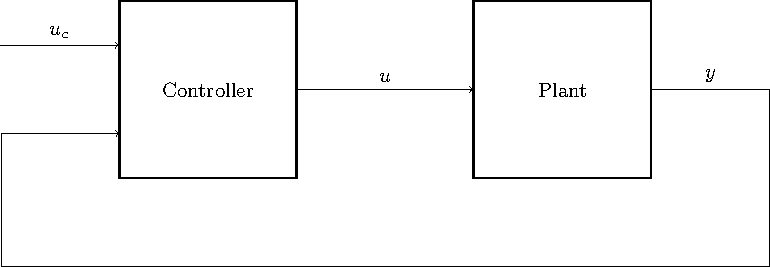
\includegraphics[width=0.6\linewidth]{2dof-block}
   \caption{Closed-loop system with two-degree-of-freedom controller}
   \label{fig:2dof}
   \end{center}
   \end{figure}
\subsection{Implement the controller}
\label{sec-1-4}

\begin{enumerate}
\item Implement the controller and the plant in Simulink. Add a disturbance signal at the output of the plant. Simulate a step-response both from the command signal and from the disturbance signal. Attach the graphs to your report.
\item Implement the controller in Simulink and interface with the true system using the Real-Time toolbox. Make a step-response and hand in the graph. What are the main differences compared to the simulated results?
\item Perform a step-response with the true system using a (much) smaller value of $a=$, for instance $a=-2$. What are the differences compared to $a=-20$?
\end{enumerate}

\end{document}
